\documentclass[]{article}

\usepackage{caption,subcaption,graphicx,float,url,amsmath,amssymb,amsthm,tocloft,cancel,mathrsfs}
\usepackage[toc,nonumberlist]{glossaries}
\usepackage{glossaries-extra,thmtools,gensymb,braket,bm,tensor}
\usepackage[toc,page]{appendix}
\usepackage[T1]{fontenc}
\usepackage[utf8]{inputenc}

\newcommand\numberthis{\addtocounter{equation}{1}\tag{\theequation}}
\newcommand{\Lagr}{\mathscr{L}}
\newtheorem{thm}{Theorem}
\newtheorem{defn}[thm]{Definition}
\newtheorem{cor}[thm]{Corollary}
\newtheorem{lemma}[thm]{Lemma}
\graphicspath{{figs/}}
\widowpenalty10000
\clubpenalty10000
\setcounter{tocdepth}{2}

%opening
\title{Theoretical Minimum\\General Relativity\\Miscellaneous Lectures}
\author{Simon Crase}

\begin{document}
	
\maketitle
	
\begin{abstract}
	These are my notes from some miscellaneous lectures related to  \emph{General Relativity}\cite{susskind2012general} lectures from Leonard Susskind's \emph{Theoretical Minimum} series\cite{susskind2007theoretical}.
\end{abstract}
	
\tableofcontents
\listoffigures
\listoftables
\listoftheorems

\section{Inside Black Holes (KITP Blackboard Lunch).}\label{sec:inh}

We are addressing a problem that's been around for 100 years: how to put together quantum mechanics and gravity?  For many years there was very little. The subject exploded with Hawking's \& Bekenstein's discovery of black hole thermodynamics. Paradoxes are very interesting; they are generally the way forward when you simply don't have anything else, when you have no experiments, no empirical data, just a set of concepts which clash. That's when we stand to learn something really new and exciting. For example, light travelling at the same speed in all frames of reference, the electron not spiralling in to nucleus, quarks being confined, the cosmological constant being 123 orders of magnitude smaller that we'd expect, the start of life.\cite{susskind2013inside}

When the paradox is solved, LS thinks we'll discover that we wee going on the right track before the paradox, but we were ignorant of some important thing.

Don't think of quantum gravity as quantizing gravity. Usual quantization has failed. Probably quantum mechanics and gravity are linked in a way which doesn't allow us to separate them. It probably doesn't make sense to take a classical theory of gravity and apply the standard rules. If this doesn't work, and there are no data, the best we can do is explore paradoxes, most of which have to do with black holes. Freeman Dyson thinks it doesn't make sense to try to fit quantum mechanics and general relativity together, as they involve different scales. LS thinks it is intolerable to have two theories that don't fit together. 

Black holes are where quantum mechanics and general relativity come together. Despite black holes being very big and very heavy, the way they contain information and interact with the rest of the world is highly quantum mechanical. Black holes seem to be the natural doorway, the place we get really surprising paradoxes from, that we can explore and hope to learn about the connection between quantum mechanics and gravity.

Let us begin with some tension that was already there in the classical theory with black holes. It's not a paradox, just a tension. The tension has to do with the difference in descriptions between outside the black hole and somebody falling in.

Figure \ref{fig:ibh-horizon} shows the dividing line between a region where there is a chance to escape, and one where there isn't. The properties of clocks and measuring rods get very distorted near the event horizon. When an observer falls in to the horizon it measures a finite time (proper time), but a distant observer will see it fall asymptotically slowly (coordinate time): this is the tension in this problem--Figure \ref{fig:ibh-minkowski}. We see an asymptotically thin observer, and everything that has fallen in form progressively thinner and thinner shells. So our picture is a thin shell, with nothing important inside, since nothing ever fell through \emph{from the perspective of a distant observer}.
\begin{figure}[H]
	\begin{center}
		\caption[Event horizon separates two regions]{Event horizon separates two regions: one where we can send light to infinity, and one where anything will end up in the singularity.}\label{fig:ibh-horizon}
		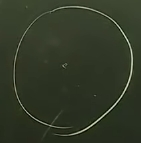
\includegraphics{ibh-horizon}
	\end{center}
\end{figure}

In a classical black hole two things are infinite for a classical black hole:
\begin{enumerate}
	\item the length of time to fall in;
	\item the amount of information you can hide in the then sedimentary structure that is on the event horizon.
\end{enumerate}

There is no limit classically on how much structure (information) you can have at the horizon of a black hole. Bits of information in classical physics can be encoded in arbitrarily weak signals of arbitrarily low energy, so these weak signals can carry any number of bits of information. There can be an infinite amount of energy hidden at the horizon, classically. Hidden information is also called \emph{entropy}.
Bekenstein did \emph{not} discover that black holes have entropy; he discovered that \emph{they do not have too much entropy}.

\begin{figure}[H]
	\begin{center}
		\caption[Consistency of times: infalling observer sees finite, external infinite.]{Consistency of times: infalling observer sees finite, external infinite. Einstein taught us that, in order to understand gravity, we should start by understanding an accelerated observer. In Minkowski space the coordinates of a constantly accelerated observer look like this. The hyperbolae represent constant position, the radial lines constant time. Notice the line for $t=\infty$. Imagine somebody falling through along curvy line. From the point of view of the falling observer only a finite proper time elapses; he doesn't care about the odd accelerated coordinates. But someone who stays outside, which involves accelerating. If you stay outside and watch someone crossing light cone it takes an infinite time, but there is nothing infinite about the perception of someone falling through. Classically this wasn't regarded as a paradox, just a curiosity. \emph{This is the structure of a black hole very near the horizon.} }\label{fig:ibh-minkowski}
		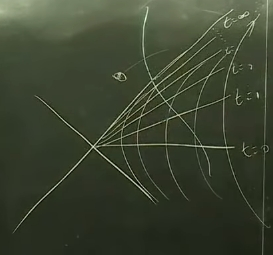
\includegraphics{ibh-minkowski}
	\end{center}
\end{figure}

Until Jacob Bekenstein\cite{wiki:jacob:bekenstein} asked the question in 1972, it was assumed that a black hole could hide an infinite amount of information; this is similar to the situation prior to quantum mechanics. In pre-quantum mechanics the radiation field of a given amount of energy could contain an infinite amount of information-- the ultraviolet catastrophe. Each mode of the radiation field, no matter what its frequency was, could store arbitrary amounts of entropy. If you had information stored classically it would migrate more and more to the ultraviolet modes, where there is an infinite phase space to contain entropy. 

The same thing would happen in Figure \ref{fig:ibh-horizon}. Entropy would cross the event horizon and, if you didn't account for it, it would seem that entropy was lost to the world. It would be absorbed by the infinitely thin layers and could not get out. This didn't feel right to Bekenstein; he suspected that black holes were like anything else and have a finite entropy.

\begin{thm}[Bekenstein]
	A black hole has a finite entropy $\propto$ area of event horizon.
\end{thm}

\begin{proof}
	Build black hole a particle at a time. A particle should contain one bit: either it is there or it isn't. But that isn't quite right. If we build black hole by sending in one bit at a time, we can't use high frequency or localized photons. A localized photon contains more information that its presence or absence; it also has information about where it might fall into the horizon. So we need a photon of a wavelength so long that we can't distinguish where it crossed the horizon.
	
	The radius of a black hole is given by:
	\begin{align*}
	R =& \frac{2 M G}{c^2} \text{. Throw in photons $\lambda\approxeq R$, one at a time.}\\
	\delta E =& \frac{hc}{\lambda} \text{, change in energy from 1 bit of information}\\
	=& \frac{hc}{R}\\
	\delta M =& \frac{\hslash}{Rc} \text{, from $E=mc^2$}\\
	\delta R =& \frac{2G}{c^2}  \frac{\hslash}{Rc}\\
	R \delta R=& \frac{2G}{c^3}  \hslash\\
	=& \delta A
	\end{align*}
	Every time you add a bit you add a fixed amount to the horizon  area. So change in area from adding one bit of information is a \emph{universal constant}.
	\begin{align*}
	S =& \frac{A c^3}{\underbrace{4}_\text{\cite{hawking1975particle}} \hslash G} \text{. Entropy.}\\
	dE =& T dS \text{. Anything with entropy and energy has temperature\cite{susskind2013statistical}}\\
	T =& \frac{\hslash  c^3}{8 \pi M k_B G} \text{. Hawking temperature--\cite{hawking1975particle}.}
	\end{align*}
\end{proof}

This has negative specific heat, as temperature goes \emph{down} with energy. Notice that in classical limit, $\hslash \rightarrow 0$, S $\rightarrow \infty$, $\rightarrow 0$. Very often quantum mechanics takes things which are infinite classically and makes them finite.

That is the description of a black hole from outside. Because it has a temperature, it radiates. The Sun radiates energy whose wavelength is small compared to the solar radius, but a black hole radiates with a wavelengths comparable to size of black hole. If you try to look at one with its own radiation it looks fuzzy. Since information is finite we have to modify our picture--see Figure \ref{fig:ibh-horizon-planck}.
\begin{figure}[H]
	\begin{center}
		\caption[Cannot store anything on a  scale smaller than Planck Length]{One way to think of Bekenstein's argument is that you cannot store anything on a vertical scale smaller than Planck Length. There is a characteristic thickness on the event horizon.}\label{fig:ibh-horizon-planck}
		\begin{subfigure}[t]{0.45\textwidth}
			\caption{ From one perspective the black hole is just a hollow sphere, the stretched event horizon, with microscopic degrees of freedom. }\label{fig:ibh-horizon-outside}
			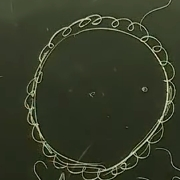
\includegraphics[width=\textwidth]{ibh-horizon-planck}
		\end{subfigure}
		\;
		\begin{subfigure}[t]{0.45\textwidth}
			\caption{Einstein's gravity suggests we should be able to fall through. Inside there could be other objects, even stars ef the black hole is big enough.}\label{fig:ibh-horizon-inside}
			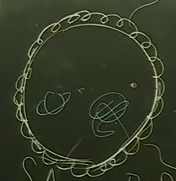
\includegraphics[width=\textwidth]{ibh-horizon-inside}
		\end{subfigure}
	\end{center}
\end{figure}
Another odd thing is that entropy is normally proportional to volume, not area: that is telling us that \emph{there is nothing inside the black hole.}
OTOH, classical black hole physics tells us that it is meaningful to fall through the horizon: it takes a finite proper time. Now we \emph{are} getting into paradox land.
\begin{itemize}
	\item From one perspective the black hole is just a hollow sphere, the stretched event horizon, with microscopic degrees of freedom--Figure \ref{fig:ibh-horizon-outside}. It is hot. Photons are redshifted so they appear cool from a distance, but event horizon is enormously hot.
	\item In all the years it took to develop these arguments, peple forgot to ask about the infalling observer. One possibility is that the black hole is just this hollow sphere with nothing inside, not even spacetime. But that isn't very satisfying, as Einstein's gravity suggests we should be able to fall through--Figure \ref{fig:ibh-horizon-inside}.
\end{itemize}

\begin{defn}[Holographic principle]
	Boundary structure functions something like a hologram. Yes, there are things on the inside, but their relationship to this structure that is holding the information about everything that ever fell through is roughly speaking a metaphor of a hologram.  The information can be thought of as being stored on the film, or the film can be thought of as a representation of the 3 dimensional reality.
\end{defn}

That is the picture as it was roughly 18 months before the date of the lecture\footnote{August 2013}.

Since event horizon is hot, it radiates heat and evaporates.

Let's come to the quantum mechanics, and what the dilemma is.

Put yourself into an infalling frame of reference. 	Infalling observer experiences empty space, and it may be entangled with something. Entanglement means that two systems are highly correlated in a quantum mechanical sense. Figure \ref{fig:ibh-horizon-alice-bob} shows Alice becoming entangled with the Hawking radiation. But there is a theorem, the monogamy of entanglement, which says that Alice can not be entangled with Bob and Hawking. 

\begin{thm}[Monogamy of entanglement]
	Monogamy of entanglement means that an entangled state cannot be shared with many parties. The more parties, the less entanglement between them. In this paper, we give a simple proof of this property and provide an upper bound of the number of parties.\cite{Yang_2006} 
\end{thm}

\begin{itemize}
	\item holographic principle requires Alice \& Bob entangled;
	\item Alice becomes entangled with distant radiation;
	\item Alice and Bob's entanglement destroyed.
\end{itemize}

\begin{figure}[H]
	\begin{center}
		\caption[Alice and Bob are entangled.]{Alice and Bob are entangled. You can find out about Alice by a Bob measurement, and vice versa. What happens when black hole evaporates? After about half evaporates, Alice is entangled with distant Hawking radiation.}\label{fig:ibh-horizon-alice-bob}
		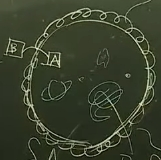
\includegraphics{ibh-horizon-alice-bob}
	\end{center}
\end{figure}
That sounds like a disaster. Breaking Alice \& Bob's entanglement will perturb nature of vacuum between interior and exterior seriously. What if interior of black hole is really encoded in distant Hawking radiation? LS doesn't like this.

One possibility is the Firewall. Once you disrupt entanglement there is no interior. It has been scooped up into Hawking radiation. There is no interior. LS doesn't like it either.

LS feels that we learn something really big from this exercise.



\begin{figure}[H]
	\begin{center}
		\caption{	Questions.}
		\begin{subfigure}[t]{0.45\textwidth}
			\caption{When stuff falls in, horizon expands  a little to meet it, then mixes up with other information in hot stretched horizon. Through holographic mapping this is equivalent to stuff actually passing through. We believe we understand this; it's the entangled stuff going out that we don't understand.}\label{fig:ibh-horizon-falling-in}
			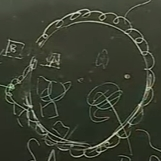
\includegraphics[width=\textwidth]{ibh-horizon-falling-in}
		\end{subfigure}
		\;
		\begin{subfigure}[t]{0.45\textwidth}
			\caption{For a sufficiently large black hole there is a region inside the event horizon that is far enough from the singularity that it is flattish. E.g. the black hole at the centre of the galaxy; someone falling in would have 20 minutes before tidal forces became a problem. You could frame the questions to refer to the outer regions. This isn't to say that the singularity isn't important, but merely that the paradox can be formulated independently of the singularity. }\label{fig:ibh-horizon-inside-large}
			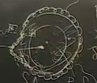
\includegraphics[width=\textwidth]{ibh-horizon-inside-large}
		\end{subfigure}
	\end{center}
\end{figure}

\section{The World As Hologram}\label{sec:hologram}
In a certain peculiar sense, the world is a hologram.  It all began from thinking about black holes. Black holes are in some sense the most exotic objects in the universe. They are dense, they are heavy, they are dangerous, but they are also ubiquitous. The universe is filled with them, and almost all the bits of information in the universe exist in black holes. So in a certain sense, although they are very exotic, they are almost everything. They contain almost all of the information in the universe.\cite{susskind2011hologram}

\begin{figure}[H]
	\caption{William Unruh's analogy for a black hole}
	\begin{subfigure}[t]{0.45\textwidth}
		\caption{Alice has become disconnected from outside: no fish can swim faster then the speed of sound.}
		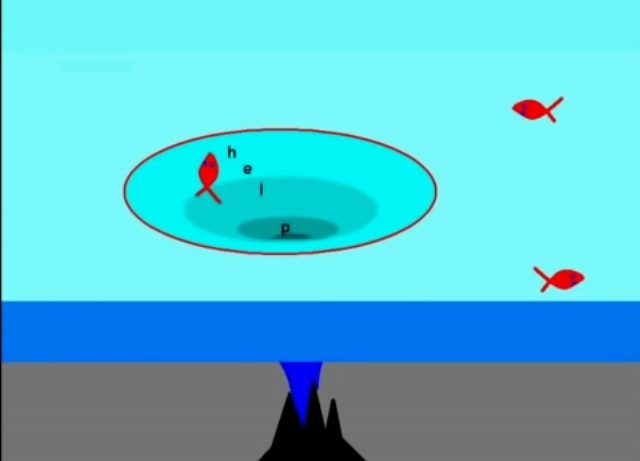
\includegraphics[width=\textwidth]{wh-alice}
	\end{subfigure}
	\begin{subfigure}[t]{0.45\textwidth}
		\caption{As you pass the event horizon, nothing bad happens to you, but you are doomed. The singularity is what is harmful, but we won't worry about that in this lecture.}
		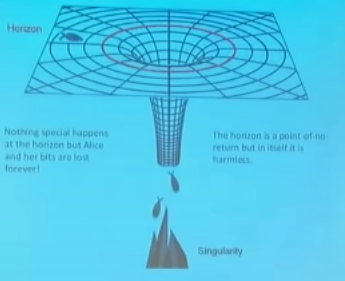
\includegraphics[width=\textwidth]{wh-black-hole}
	\end{subfigure}
\end{figure} 

Information comes in bits: ''King Canute had warts on his chin''. Physicists aren't interested in the meaning, just the symbols.

\begin{figure}[H]
	\begin{center}
		\caption{''King Canute had warts on his chin''--Morse code. 65 bits.}
		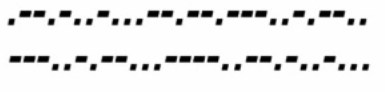
\includegraphics[width=0.6\textwidth]{wh-kcwc}
	\end{center}
\end{figure}

\begin{defn}[$-1^{st}$ law of physics]
	Bits of information are indestructible: distinctions between situations, distinction between configurations are never erased; they never disappear from the world..
\end{defn}

Figure \ref{fig:conflict} summarizes Hawking's central point from 1976: on one hand information is indestructible, on the other Bob sees Alice's bits disappearing as she crosses the event horizon.
\begin{figure}[H]
	\caption{Conflict of principles: a paradox.}\label{fig:conflict}
	\begin{subfigure}[t]{0.45\textwidth}
		\caption{Information is indestructible. Bits are forever. They are not just bits of information: they are also bits of energy.}
		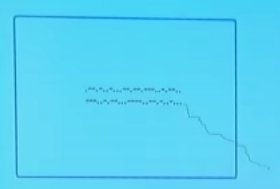
\includegraphics[width=\textwidth]{wh-kcwc-1st}
	\end{subfigure}
	\;
	\begin{subfigure}[t]{0.45\textwidth}
		\caption{Once Alice crosses the event horizon, as far a Bob is concerned her bits have disappeared from the world.}
		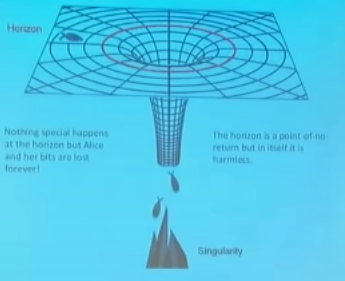
\includegraphics[width=\textwidth]{wh-black-hole}
	\end{subfigure}
\end{figure}

But black holes evaporate....The evaporate photons and stuff, shrinking to a tiny black hole before disappearing. Where is Alice? Where are her bits? They can't have escaped from the horizon, because otherwise they'd have to exceed the speed of light. We have a conflict of principle.

\begin{figure}[H]
	\caption{Entropy--Information that is hidden.}
	\begin{subfigure}[t]{0.45\textwidth}
		\caption{Bathtub of hot water. How much information to we need? Temperature and volume}
		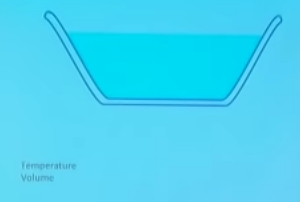
\includegraphics[width=\textwidth]{wh-bathtub}
	\end{subfigure}
	;\
	\begin{subfigure}[t]{0.45\textwidth}
		\caption{Hidden Information, positions and velocities of molecules, stored in a huge number of degrees of freedom.}
		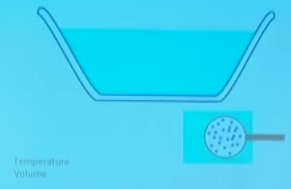
\includegraphics[width=\textwidth]{wh-bathtub-detail}
	\end{subfigure}
\end{figure}

Jacob Bekenstein--Black holes have information (1972). Everybody knows that, but Bekenstein worked out how much information was hidden. He considered the process of building a black hole by dropping particles in, and found the number of hidden bits of information is equal to the area of the event horizon, measured in Planck units: one Planck area $=\frac{\hslash G}{c^3}$. Think of bits an impenetrable objects covering event horizon.


\begin{figure}[H]
	\begin{center}
		\caption{Information on event horizon}
		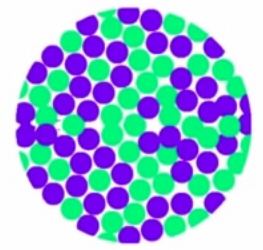
\includegraphics{wh-info-event-horizon}
	\end{center}
\end{figure}

What are the hidden microscopic structures that make up the horizon of a black hole? There must be hidden degrees of freedom that are making up that entropy.

\begin{figure}[H]
	\caption{String Theory is a theory where elementary particles are tiny pieces of string}
	\begin{subfigure}[b]{0.3\textwidth}
		\caption{Adding more energy makes the string more tangled.}
		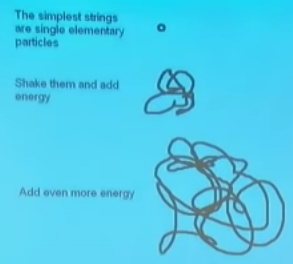
\includegraphics[width=\textwidth]{wh-strings}
	\end{subfigure}
	\;
	\begin{subfigure}[b]{0.3\textwidth}
		\caption{If string so tangled we can't follow it, because we are too large or not smart enough, we say it has entropy. It is not yet a black hole. If we have enough string, however, gravity will pull it together into a black hole.}
		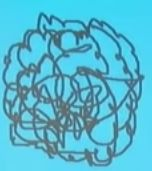
\includegraphics[width=\textwidth]{wh-string-tangle}
	\end{subfigure}
	\;
	\begin{subfigure}[b]{0.3\textwidth}
		\caption{Metaphorically we are left with little pieces of string hanging out of the horizon. They comprise the degrees of freedom that carry entropy.}
		
\includegraphics[width=\textwidth]{wh-string-hanging-out}
	\end{subfigure}
\end{figure}

LS is not here to sell string theory. Whatever the entropy of black holes is, it is something which is very small, very chaotic, and in a constant state of agitated motion. Motion and entropy mean heat, so the surface is a flat, two dimensional soup of bits.

\begin{figure}[H]
	\begin{center}
		\caption[Measuring the Temperature of Event Horizon]{Measuring the Temperature of Event Horizon: a conflict of principle. Remember Alice, who happily sailed through the point of no return ''cool as a cucumber''? Or was she thermalized and sent back as photons?}
		\begin{subfigure}[t]{0.2\textwidth}
			\caption{Measuring the Temperature of Event Horizon}
			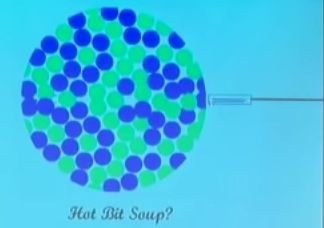
\includegraphics[width=\textwidth]{wh-hot-bit-soup}
		\end{subfigure}
		\;
		\begin{subfigure}[t]{0.2\textwidth}
			\caption{Hot bit soup?}
			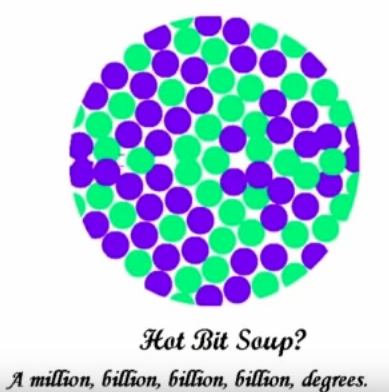
\includegraphics[width=\textwidth]{wh-really-hot}
		\end{subfigure}
		\;
		\begin{subfigure}[t]{0.2\textwidth}
			\caption{Or a harmless point of no return?}
			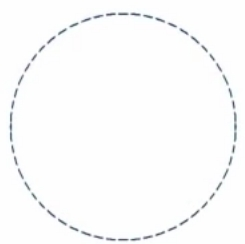
\includegraphics[width=\textwidth]{wh-or-harmless}
		\end{subfigure}
		\begin{subfigure}[t]{0.2\textwidth}
			\caption{Thermalized Alice}
			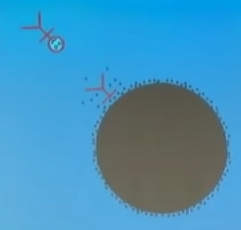
\includegraphics[width=\textwidth]{wh-thermal-alice}
		\end{subfigure}
	\end{center}
\end{figure}

Which picture is true? Both are true.

\begin{figure}[H]
	\begin{center}
		\caption[Conflict of Principle]{Conflict of Principle. Bob doesn't see Alice fall through horizon, but he does see radiation--Alice's bits.}
		\begin{subfigure}[t]{0.45\textwidth}
			\caption{Alice thinks she passes safely}
			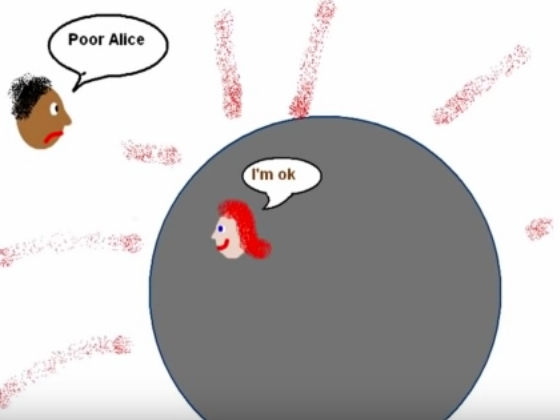
\includegraphics[width=\textwidth]{wh-conflict-alice-bob}
		\end{subfigure}
		\;
		\begin{subfigure}[t]{0.45\textwidth}
			\caption{Just before Alice passes the horizon Bob looks at her, i.e. shine photons on her and asks whether she is being thermalized. In order to do this he has to hit here with enough energetic photons that she will be thermalized!}\label{fig:wh-bobs-pov}
			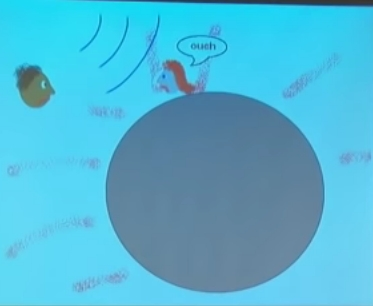
\includegraphics[width=\textwidth]{wh-bobs-pov}
		\end{subfigure}
	\end{center}
\end{figure}

There is no operational conflict, as Alice cannot get the message to Bob, but the situation seems unsatisfactory. Let's see if we can push the experiment a little further--Figure \ref{fig:wh-bobs-pov}. Quantum mechanics is always like that: you try to show that something doesn't happen by doing an experiment, and the experiment makes it happen!

This still isn't satisfying! Something deep is going on here, about information.
There are two representations of the same reality: the 3 dimensional representation of Alice passing through, and the 2 dimensional representation in shich she is thermalized.

\begin{figure}[H]
	\begin{center}
		\caption[A painting is a 2D representation of a 3D scene]{A painting is a 2D representation of a 3D scene. Familiarity with the way people look, etc, creates a 3D fiction in our brains! We can't tell whether cadaver is short, because paint is just 2D. The text on the plaque can't be read. The 3D information isn't there.}
		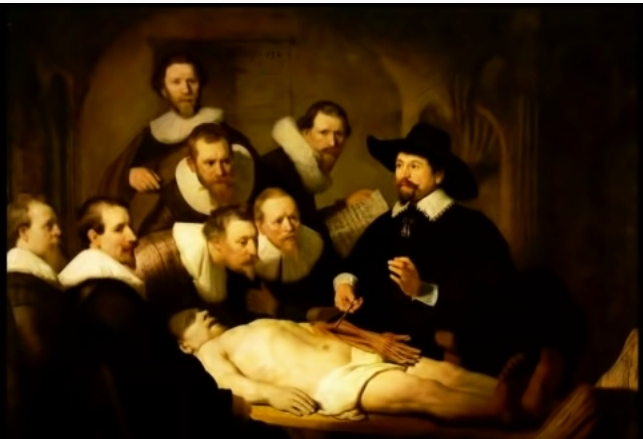
\includegraphics[width=0.8\textwidth]{wh-painting}
	\end{center}
\end{figure}



\begin{figure}[H]
	\caption{Coding 2D and 3D information with bits.}
	\begin{subfigure}[t]{0.45\textwidth}
		\caption{Painting as pixels}
		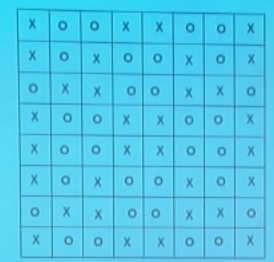
\includegraphics[width=\textwidth]{wh-painting-pixels}
	\end{subfigure}
	\begin{subfigure}[t]{0.45\textwidth}
		\caption{Room as voxels}
		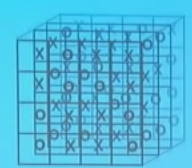
\includegraphics[width=\textwidth]{wh-voxels}
	\end{subfigure}
\end{figure}

What about 3D? Divide room into voxels the size of atoms--pretend there is only one kind of atom. Then we can describe state by whether or not there is an atom in each voxel. Then we can represent the room by bits.

Can it be that our world, or at least the surface of a black hole, can be described in both 2D and 3D? You can represent 3D data in 2D, but the result is always to scramble it horribly. An example is a hologram, i.e. the piece of film.

\begin{figure}[H]
	\caption[Hologram compresses image from 3D to 2D]{Hologram compresses image from 3D to 2D, but also scrambles it beyond recognition--unless you know detailed code.}
	\begin{subfigure}[t]{0.45\textwidth}
		\caption{A piece of holographic film}
		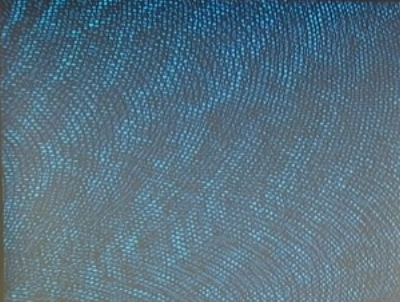
\includegraphics[width=\textwidth]{wh-holographic-film}
	\end{subfigure}
	\;
	\begin{subfigure}[t]{0.45\textwidth}
		\caption{Shine light to show image. You can walk around to see hair on back of head. Hologram doesn't contain information on what is inside head, but could make hologram from MRI scan and encode all 3D information}
		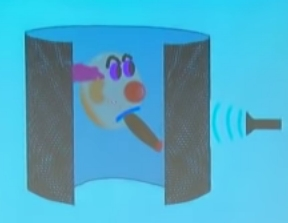
\includegraphics[width=\textwidth]{wh-3d-image}
	\end{subfigure}
\end{figure}
So a black hole horizon is like a hologram representing everything that is inside. We have two representations of the same reality.

\begin{figure}[H]
	\begin{center}
		\caption[Two representations of the same reality]{Two representations of the same reality; the hot bit soup encodes the same data as Alice gets falling through the horizon.}
		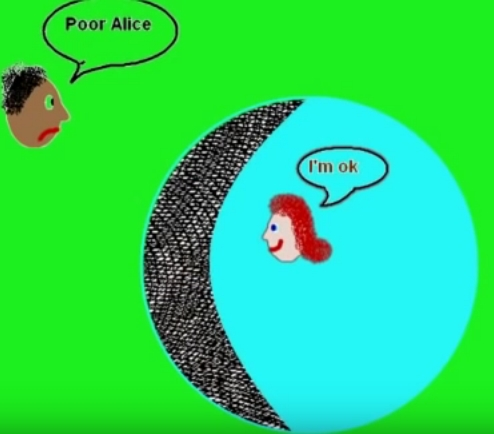
\includegraphics[width=0.6\textwidth]{wh-2reps}
	\end{center}
\end{figure}

It is not just black holes. In a certain sense the entire universe can be represented as a hologram, or any finite region of the universe can be represented as a hologram in essentially the same way. I

\begin{figure}[H]
	\begin{center}
		\caption{The Universe}
		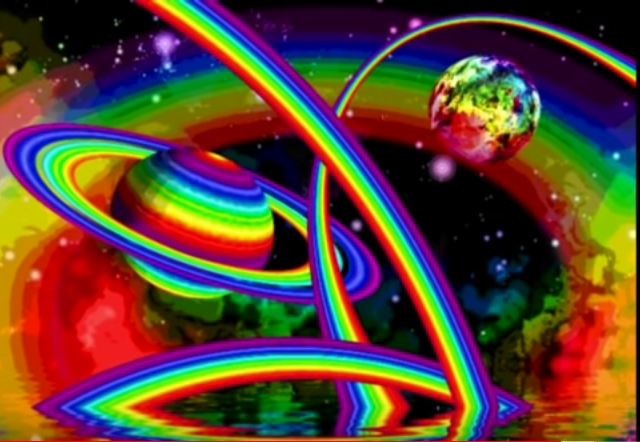
\includegraphics[width=0.8\textwidth]{wh-universe}
	\end{center}
\end{figure}

\begin{figure}[H]
	\begin{center}
		\caption[Put some information in a box]{Put some information in a box. It could be alphabet soup, wine, cheese,...}
		\begin{subfigure}[t]{0.45\textwidth}
			\caption{	What is the maximum amount of information that you can put in?}
			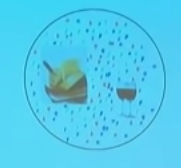
\includegraphics[width=0.8\textwidth]{wh-information-in-box}
		\end{subfigure}
		\begin{subfigure}[t]{0.45\textwidth}
			\caption{Surround with a shell, then squeeze, so it collapses into a black hole. If the $-1^{st}$ law is correct, then all the original information is hidden in the black hole--and we know how much this is: the area of the horizon in Planck units!}
			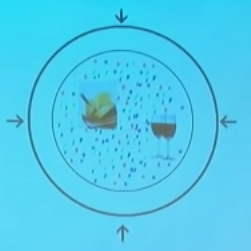
\includegraphics[width=0.8\textwidth]{wh-surround-region}
		\end{subfigure}
	\end{center}
\end{figure}
The maximum about of information that can be held in a room is proportional to the area of the walls! The world is pixelated, not voxelated.
\begin{defn}[The holographic principle]
	The maximum amount of information in a region of space is proportional to the area of the region.
\end{defn}

There are other kinds of horizon in cosmology.

\begin{figure}[H]
	\begin{center}
		\caption[Imagine the Universe as a lake filled with fish]{Imagine the Universe as a lake filled with fish, Alice, Bob, and Charlie. There are pipes bringing in new water. This causes the puddle to expand. Imagine that it follows Hubble's Law (accelerated expanding universe): the further apart two fish are, the faster they will be separating. }
		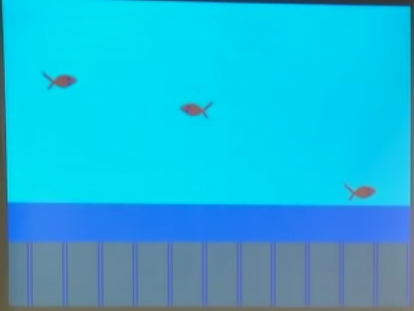
\includegraphics[width=0.6\textwidth]{wh-cosmology-fish}
	\end{center}
\end{figure}

\begin{figure}[H]
	\caption{Alice and Bob are communicating, but they are separating.}
	\begin{subfigure}[t]{0.45\textwidth}
		\caption{There is an event horizon, which we'll call an external horizon}
		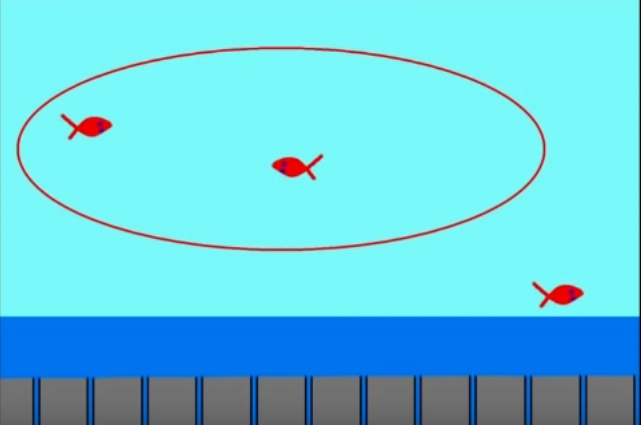
\includegraphics[width=\textwidth]{wh-cosmology1}
	\end{subfigure}
	\begin{subfigure}[t]{0.45\textwidth}
		\caption{Event Horizon has been crossed}
		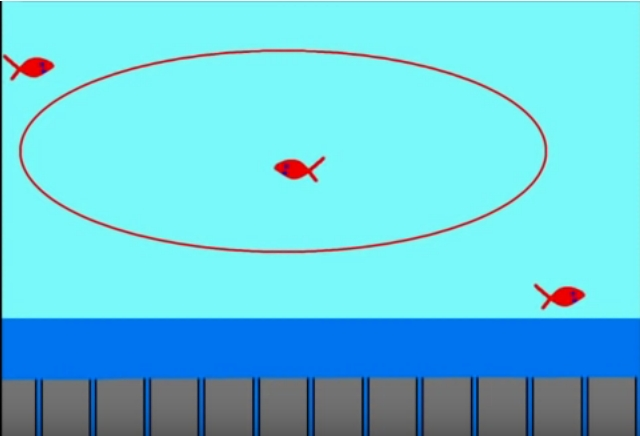
\includegraphics[width=\textwidth]{wh-cosmology2}
	\end{subfigure}
\end{figure}

The Universe is expanding, exactly as if new space were flowing in, and each person has a horizon, which is moving slower than the speed of light. It looks as if most of the world is beyond all possible observation. We know that the Universe is at least 1000 times larger, by volume, than we can ever see.

\begin{itemize}
	\item The Universe is at least 1000 times larger, by volume, than the region we can ever see. The rest is beyond our horizon.
	\item What is the meaning of the stuff we can never detect?
	\item How can we confirm it by real observation?
	\item What is the proper description of a world that is bigger than the cosmic horizon?
	\item Is our cosmic horizon a 2 dimensional scrambled hologram of all that lies beyond it? 
\end{itemize}

\section{Complexity and Gravity }

You can't really prove anything in complexity. You can conjecture this, and prove it is the same as some other conjecture, but it is extremely difficult to prove anything in complexity.\cite{susskind2018complexity}

LS technique for doing physics: close your eyes, try to visualize the answer, then say what it is. Visualize the phenomenon, the try to visualize a collection of phenomena which are related in some way, and tend to reinforce the same view, until you come to the conclusion that is this were wrong so many other things would have to be wrong that there would be big problems.

The connection between complexity and black holes is highly improbable; after many years of thinking about it, LS concludes there is no alternative. It has to be right, although the precise form in which it is true has still to be given.

You don't understand quantum gravity until you understand the interior of black holes; you don't understand black holes until you understand horizons.

Why is complexity important in QM? Feynman pointed out that Hilbert Space is enormous. It is much bigger than spaces for classical problems.



Start with $K$ qbits,  a $2^K$ dimensional state space, so state is:
\begin{align*}
	\ket{\psi}=\sum_{i=1}^{2K}\alpha_i \ket{i}
\end{align*}
How big is this space? It is a continuous infinity, so let us regularise the $\alpha_i$ by picking them from some discrete set $\{\alpha_1, \alpha_m\}$. We than have $m^{2^k}$ states--$\#s$, say, which grows very fast.

\begin{align*}
	\ln \#s =& 2^K \ln m \text{--remember this pattern!} \numberthis \label{eq:pattern}
\end{align*}

This is strongly sensitive to $K$, but weakly sensitive to $m$ (cutoff parameter).

Let's try to do more precise counting. What is the space of states of a $K$ qbit system? $CP(N)$, where $N=2^K$. Again we'll regularize it: fill hypersphere with $\epsilon$-balls. We coarse grain, and identify states with $\epsilon$-balls. Calculate volume:
\begin{align*}
	V_{CP}=& \frac{\pi^N}{N!} \text{, where $N=2^K$. Now volume $\epsilon$-ball is}\\
	V_B =& \frac{\pi^N}{N!} \epsilon^{2N} \text{, because real dimensionality is $2N$}\\
	\#s =& \bigg(\frac{1}{\epsilon}\bigg)^{2(2^K-1)} \text{, coarse graining}\\
	\ln \#s \approx & 2^K \ln \frac{1}{\epsilon} \text{, same pattern as (\ref{eq:pattern} -- strong dependence on $K$, weak dependence on regulator)}
\end{align*}

How far apart can states be in this space? What is the diameter, and the distance between states. One notion is inner product distance.

\begin{align*}
	d_{AB}=&\arccos \left|\braket{A|B}\right| \text{, with thie metric distance is small}\\
	d_{AB}<&\frac{\pi}{2}
\end{align*}
On the other hand, that seems a little ridiculous. It doesn't show all the difference between states. The other notion is \emph{relative complexity,} the number of small steps from one to the other, which bring us to the idea of a \emph{quantum circuit}.


\begin{align*}
	\ket{A} =& g_1 g_2 ... g_n \ket{B} \text{, where $g_i$ are single gates}
\end{align*}

\begin{defn}[Universal gates]
	A universal collection of gates is one that allows us to get from any $\epsilon$-ball to another.
\end{defn}

\begin{defn}[Relative complexity]
	The relative complexity of A and B, $\mathscr{C}$, is the minimum $n$ such that $\ket{A} =g_1 g_2 ... g_n \ket{B}$.
\end{defn}

This is the shortest path from A to B (in units of gates), so it is a geodesic with the right definition of distance. It is a \emph{metrical notion}. LS says this is a theme of the lecture, and that he considers it to be the right way to think about complexity.
 


Now lets talk about unitary matrices. We can think of one as an operator, or as a maximally entangled state of two systems.
\begin{align*}
	U =& U_{ij}\ket{i}\bra{j} \text{, operator}\\
	\ket{V} =& V_{ij}\ket{i} \ket{\bar{j}}
\end{align*}
When we talk about distance between operators we are also talking about distance between maximally entangled states.

There are $2^{2K}$ matrix elements (number of constraints for unitary is much smaller), so $m^{2^{2K}}$ unitaries. Let's do an $\epsilon$-ball calculation. First calculate the unitary group of dimension $2^K$, then calculate the volume of an $\epsilon$-ball and divide.
\begin{align*}
	\#unitaries =& \bigg(\frac{2^K}{\epsilon^2}\bigg)^\frac{4K}{2}\\
	\ln \#unitaries =& 4^K\bigg(\frac{K \ln K}{2} + \ln\frac{1}{\epsilon}\bigg)\\
	\approx 4^K
\end{align*}

Distance between unitaries.

\begin{align*}
	d_{UV}=& \arccos \left|Tr(U^\dagger V)\right|\\
	\mathcal{C}_{UV}=& min_n \{U=g_n...g_1V\}
\end{align*}
\url{https://youtu.be/6OXdhV5BOcY?t=1732}

\section{Why is Time a One Way Street?}

Lecture given at the Santa Fe Institute.\cite{susskind2013why}

Why is it so much easier to know what the past is than to know what the future is? The ancients would have said that events in the past have happened, things in the future haven't happened yet.

The second law of thermodynamics is the archetypal illustration of time being a one way street.Newtons Laws don't contain this sort of asymmetry. If Einstein is right about space-time, why is time a one way street when x and y are not?

Entropy \emph{almost always} increases--Ludwig Boltzmann.

Boltzmann's Universe in a Box.
\begin{itemize}
	\item  In a completely empty universe, nothing happens.
	\item Imagine we start in a very special configuration, e.g. everything in one corner--Figure \ref{fig:bolztmann-start}-- and let stuff flow--Figure \ref{fig:one_way_street-Boltzmann}--which is what happens \emph{almost all} of the time. During the time that the structure is there, everything interesting in the universe must have happened.
	\item Wait long enough and all you have is particles in thermal equilibrium--Figure \ref{fig:end-game-thermal-equilibrium}. We end up with a boring configuration where nothing interesting ever happens again.
\end{itemize}

\begin{figure}[H]
	\begin{center}
		\caption{Matter evolving from initial configuration}
		\begin{subfigure}[b]{0.3\textwidth}
			\caption{Matter concentrated in special initial state}\label{fig:bolztmann-start}
			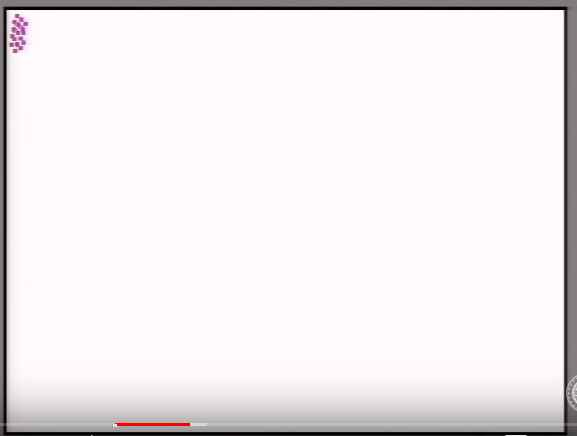
\includegraphics[width=\textwidth]{bolztmann-start}
		\end{subfigure}
		\;
		\begin{subfigure}[b]{0.3\textwidth}
			\caption{Matter streaming out and eddying}\label{fig:one_way_street-Boltzmann}
			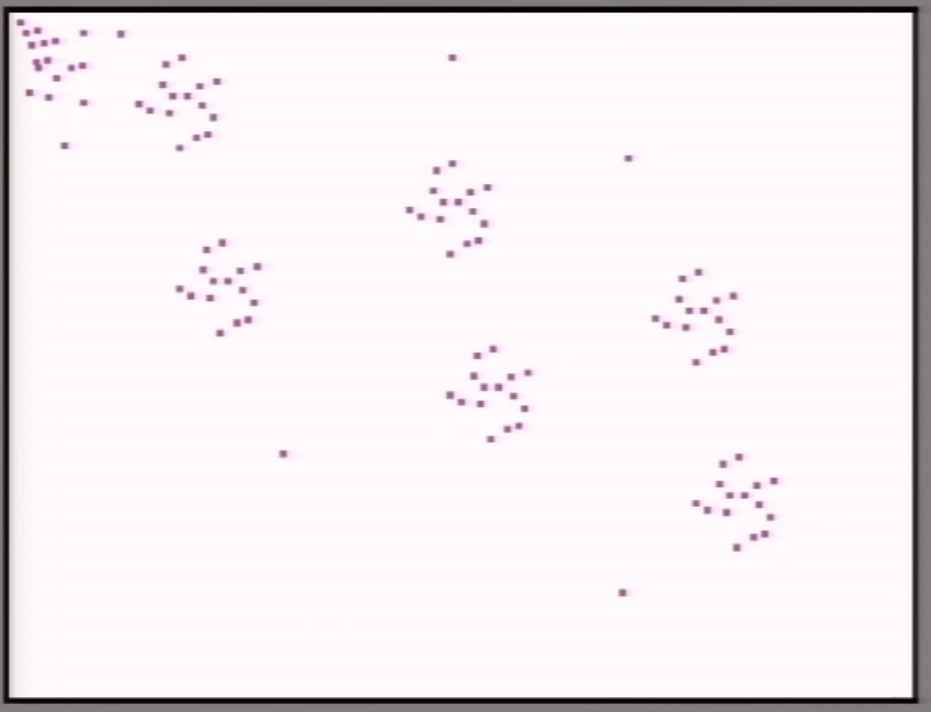
\includegraphics[width=\textwidth]{one_way_street-Boltzmann}
		\end{subfigure}
		\;
		\begin{subfigure}[b]{0.3\textwidth}
			\caption{Boring Thermal Equilibrium}\label{fig:end-game-thermal-equilibrium}
			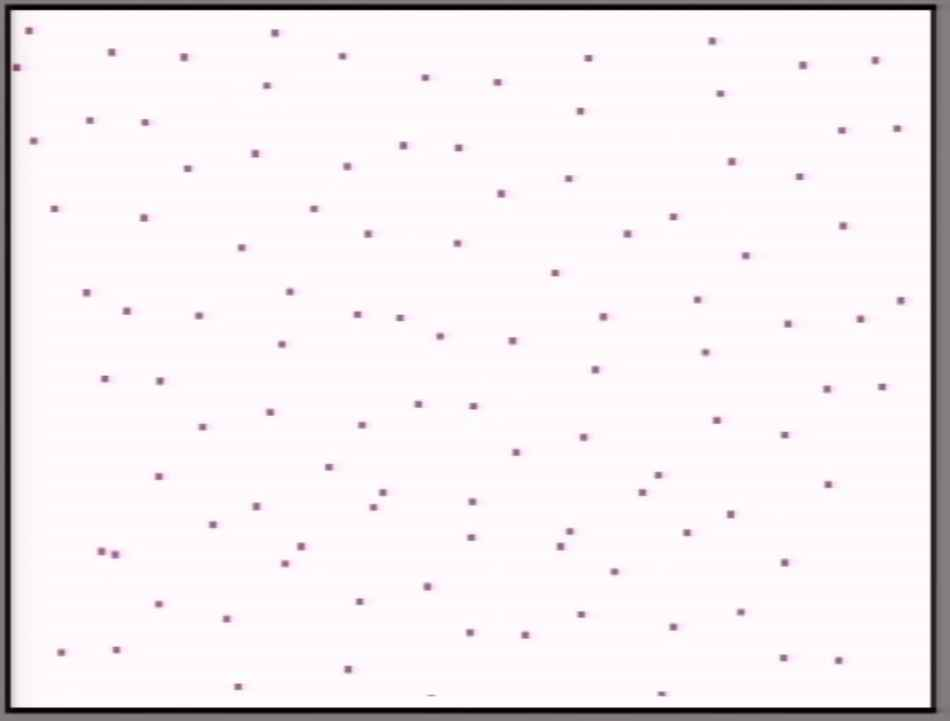
\includegraphics[width=\textwidth]{end-game-thermal-equilibrium}
		\end{subfigure}
	\end{center}
\end{figure}

Boltzmann knew this wasn't quite right. If you wait long enough the particles will originally assemble in the corner again--Figure \ref{fig:bolztmann-start}--then Figure \ref{fig:one_way_street-Boltzmann}. Figure \ref{fig:end-game-thermal-equilibrium} is not the end game after all, just the end game for a long, long time. These things are called Poincar\'e Recurrences. 

\begin{figure}[H]
	\caption{Configuration Space}
	\begin{subfigure}[b]{0.3\textwidth}
		\caption{Space of all possible configurations: blue region represents all coordinates where there is interesting stucture, e.g. galaxies, planets, birds; little pink dot the very special configuration; white is boring equilibrium. System evolves from starting configuration through interesting configurations to boring.}
		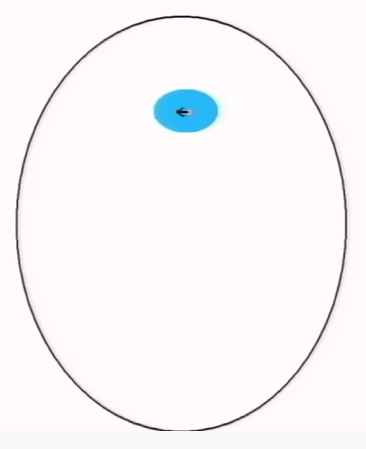
\includegraphics[width=\textwidth]{time-config-space}
	\end{subfigure}
	\;
	\begin{subfigure}[b]{0.3\textwidth}
		\caption{If you wait long enough, Universe will pass through every possible state.  Now and then it will go through blue region occasionally without going through pink, but sometime pink also. In the blue region plants and galaxies can exist, but we usually don't go through special starting region.}\label{fig:time-univers-passes-through-every-possible-state}
		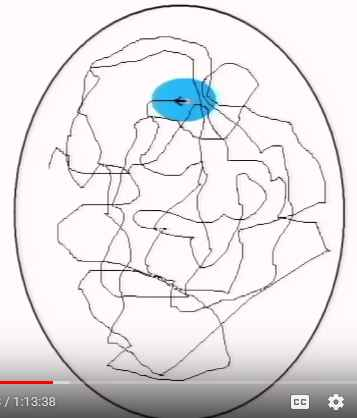
\includegraphics[width=\textwidth]{time-univers-passes-through-every-possible-state}
	\end{subfigure}
	\;
	\begin{subfigure}[b]{0.3\textwidth}
		\caption{This is how a universe built from fluctuation might look.}\label{fig:time-universe-from-fluctuation}
		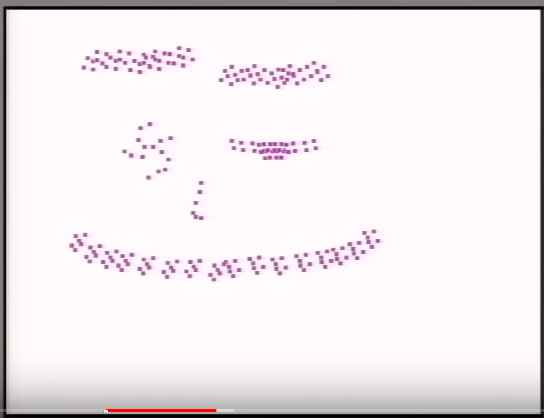
\includegraphics[width=\textwidth]{time-universe-from-fluctuation}
	\end{subfigure}
\end{figure}

Figure \ref{fig:time-univers-passes-through-every-possible-state} that, most often, if you get a world that looks like ours, the past won't look like our past. Most of the time the universe won't look like it flowed out of the corner, i.e. the Big Bang. Most universes that are created out of fluctuation don't look recognizable--Figure \ref{fig:time-universe-from-fluctuation}. \emph{Boltzmann therefore rejected this as a possible explanation of the world.} Only the first time that the universe drops out of a corner do we get stars and galaxies; most other times we get random garbage, but good enough to live in. You don't see the Big Bang, but something random.

The modern version of Boltzmann's question is: what is the most likely configuration for the universe, given that it contains intelligence and is able to ask questions such as ''what is the most likely configuration...''? The most likely thing is a brain and nothing else--Figure \ref{fig:t1ws-brain}.

\begin{figure}[H]
	\begin{center}
		\caption[The most likely thing is a brain and nothing else]{The most likely thing is a brain and nothing else, because to make 2 brains is much less likely.}\label{fig:t1ws-brain}
		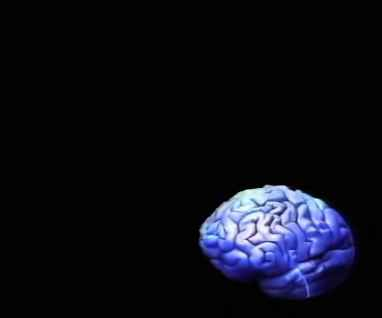
\includegraphics[width=0.6\textwidth]{t1ws-brain}
	\end{center}
\end{figure}

Physicists call Figure \ref{fig:t1ws-brain} a Boltzmann Brain. This isn't the right theory of the world, as we don't see this.

\begin{itemize}
	\item It is very unlikely that we live in a Boltzmann's Box;
	\item What does cosmology have to say about it?
	\item What we want is a "one-shot" universe with a very special starting point. It does its own thing, and thee is no chance of recurrences.
\end{itemize}
You still have a problem understanding why the molecules started in a very special configuration, but maybe one day we'll understand that.


Twenty five years ago we had two types of Big Bang cosmology, Open and Closed --Figures \ref{fig:wt1ws-closed-universe} and \ref{fig:wt1ws-openuniverse}. They are both one-shot universes, but we need to understand the starting point. 

\begin{figure}[H]
	\caption{Twenty five years ago we had two types of Big Bang cosmology}
	\begin{subfigure}[t]{0.45\textwidth}
		\caption{Closed Universe (Big Crunch)}\label{fig:wt1ws-closed-universe}
		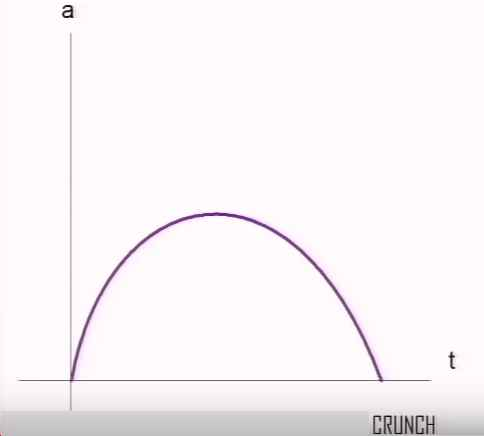
\includegraphics[width=\textwidth]{wt1ws-closed-universe}
	\end{subfigure}
	\begin{subfigure}[t]{0.45\textwidth}
		\caption{Open Universe}\label{fig:wt1ws-openuniverse}
		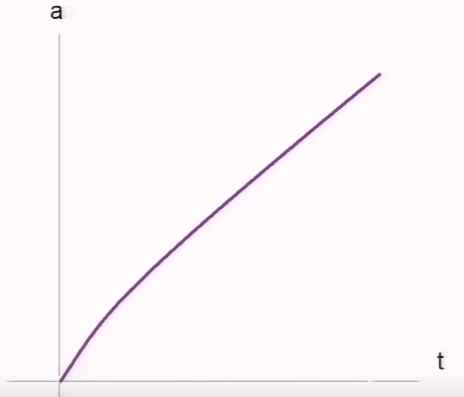
\includegraphics[width=\textwidth]{wt1ws-openuniverse}
	\end{subfigure}
\end{figure}

Then they discovered dark energy--$\Lambda$. This can have two effects:
\begin{enumerate}
	\item \emph{either} $\Lambda>0$, which accelerates the expansion--Figure \ref{fig:wt1ws-lambda-plus};
	\item \emph{or} $Lambda<0$, which accelerates the crunch--Figure \ref{fig:wt1ws-lambda-minus}.
\end{enumerate}

\begin{figure}[H]
	\caption{Effect of $\Lambda$, the Cosmological Constant}
	\begin{subfigure}[t]{0.45\textwidth}
		\caption{ $\Lambda>0$}\label{fig:wt1ws-lambda-plus}
		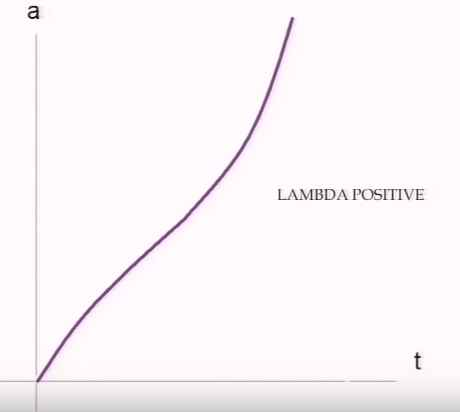
\includegraphics[width=\textwidth]{wt1ws-lambda-plus}
	\end{subfigure}
	\begin{subfigure}[t]{0.45\textwidth}
		\caption{ $\Lambda<0$}\label{fig:wt1ws-lambda-minus}
		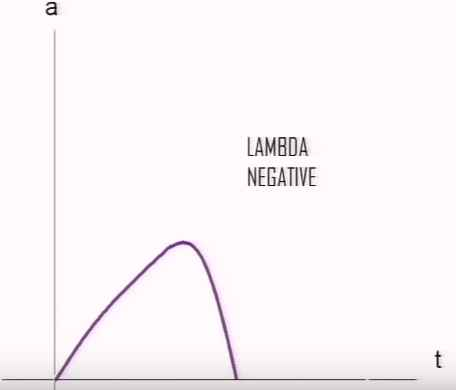
\includegraphics[width=\textwidth]{wt1ws-lambda-minus}
	\end{subfigure}
\end{figure}

These both sound like good candidates for a one-shot universe. In our universe  $\Lambda>0$ (observed), which sounds like a one-shot universe.

\url{https://youtu.be/jhnKBKZvb_U?t=2232}

\bibliographystyle{unsrt}
\addcontentsline{toc}{section}{Bibliography}
\raggedright
\bibliography{tm}

\end{document}
